
%\noindent
\justifying
\setlength{\parskip}{1em}

In the last decades, the field of computer vision has made a tremendous amount of progress, especially in the field of domain adaptation. Numerous image-to-image translation methods are invented and are improved significantly, \acp{GAN} were among them\cite{pang2021imagetoimage}. Further, several variants of \acp{GAN} are evolved over the years to resolve various problems. This chapter aims to discuss different image-to-image translation methods. Also, a brief theoretical comparison of existing methods is carried out in section \ref{rwdiscussion}. Finally, section \ref{rwconclusion} concludes the motivation behind choosing the proposed approach of this thesis.

\section{Literature Survey}\label{LiteratureSurvey}


Ian J. Goodfellow et al.\cite{goodfellow2014generative} proposed a framework of \acp{GAN} in which two models are simultaneously trained. ``A generative model is trained to learn the data distribution, and a discriminative model that predicts the probability that a sample came from the training data rather than a generative model. The idea of training a generative model is to generate realistic data and maximize the probability of a discriminative model making a mistake. The generator learns to generate realistic data, and the discriminator learns to distinguish real data from the generator's fake data. The generator is penalized by the discriminator for producing non-credible results. As training starts, the generator begins to create fake data, and the discriminator quickly learns to classify that it's fake and the generator is penalized to improve and produce credible results. The generator gets closer to producing output samples that can fool the discriminator as training progresses. Finally, if generator training goes well, the discriminator becomes worse at distinguishing between real and fake samples.  At the end of the training, ultimately, we have a generator model which produces credible results which are similar to real data''\cite{goodfellow2014generative}. Authors have trained \ac{GAN} on a range of datasets including MNIST\cite{726791}, the Toronto Face Database (TFD)\cite{susskind2010toronto}, and CIFAR-10\cite{krizhevsky2009learning}, also compared against already existing methods like \ac{DBN}\cite{bengio2012better}, \ac{Stacked-CAE}\cite{bengio2012better}, and \ac{Deep-GSN}\cite{bengio2014deep}. The authors do not claim that ``the samples generated by \acp{GAN} are better than samples generated by already existed methods''\cite{goodfellow2014generative}. Authors believe ``at least the obtained results are competitive when compared with the better generative models in the literature, which highlights the potential of the generative adversarial framework''\cite{goodfellow2014generative}. ``The first and foremost advantage of \acp{GAN} is computation when compared to other generative models. Adversarial models may have added statistical advantage from the generator network being updated by the gradients flowing through the discriminator using backpropagation, not being updated directly with data examples''\cite{goodfellow2014generative}. Backpropagation is an algorithm to calculate gradients of the loss function to update weights of the neurons in the neural network\cite{goodfellow2017deep}. Authors metioned, to prevent the Helvetica Scenario\cite{manisha2019generative}, special care must be taken while training the \acp{GAN}. The generator must not be trained too much without updating the discriminator, training of both models should happen simultaneously. The discriminator must be updated well to provide maximum error to update the generator to produce high-quality images. In the Helvetica Scenario, the generator collapses, repeatedly producing the same output or a small set of outputs. Usually, \acp{GAN} should produce a wide variety of outputs. The Helvetica Scenario is also called Mode Collapse\cite{thanhtung2020catastrophic}.

\begin{figure}
        \begin{center}
 	    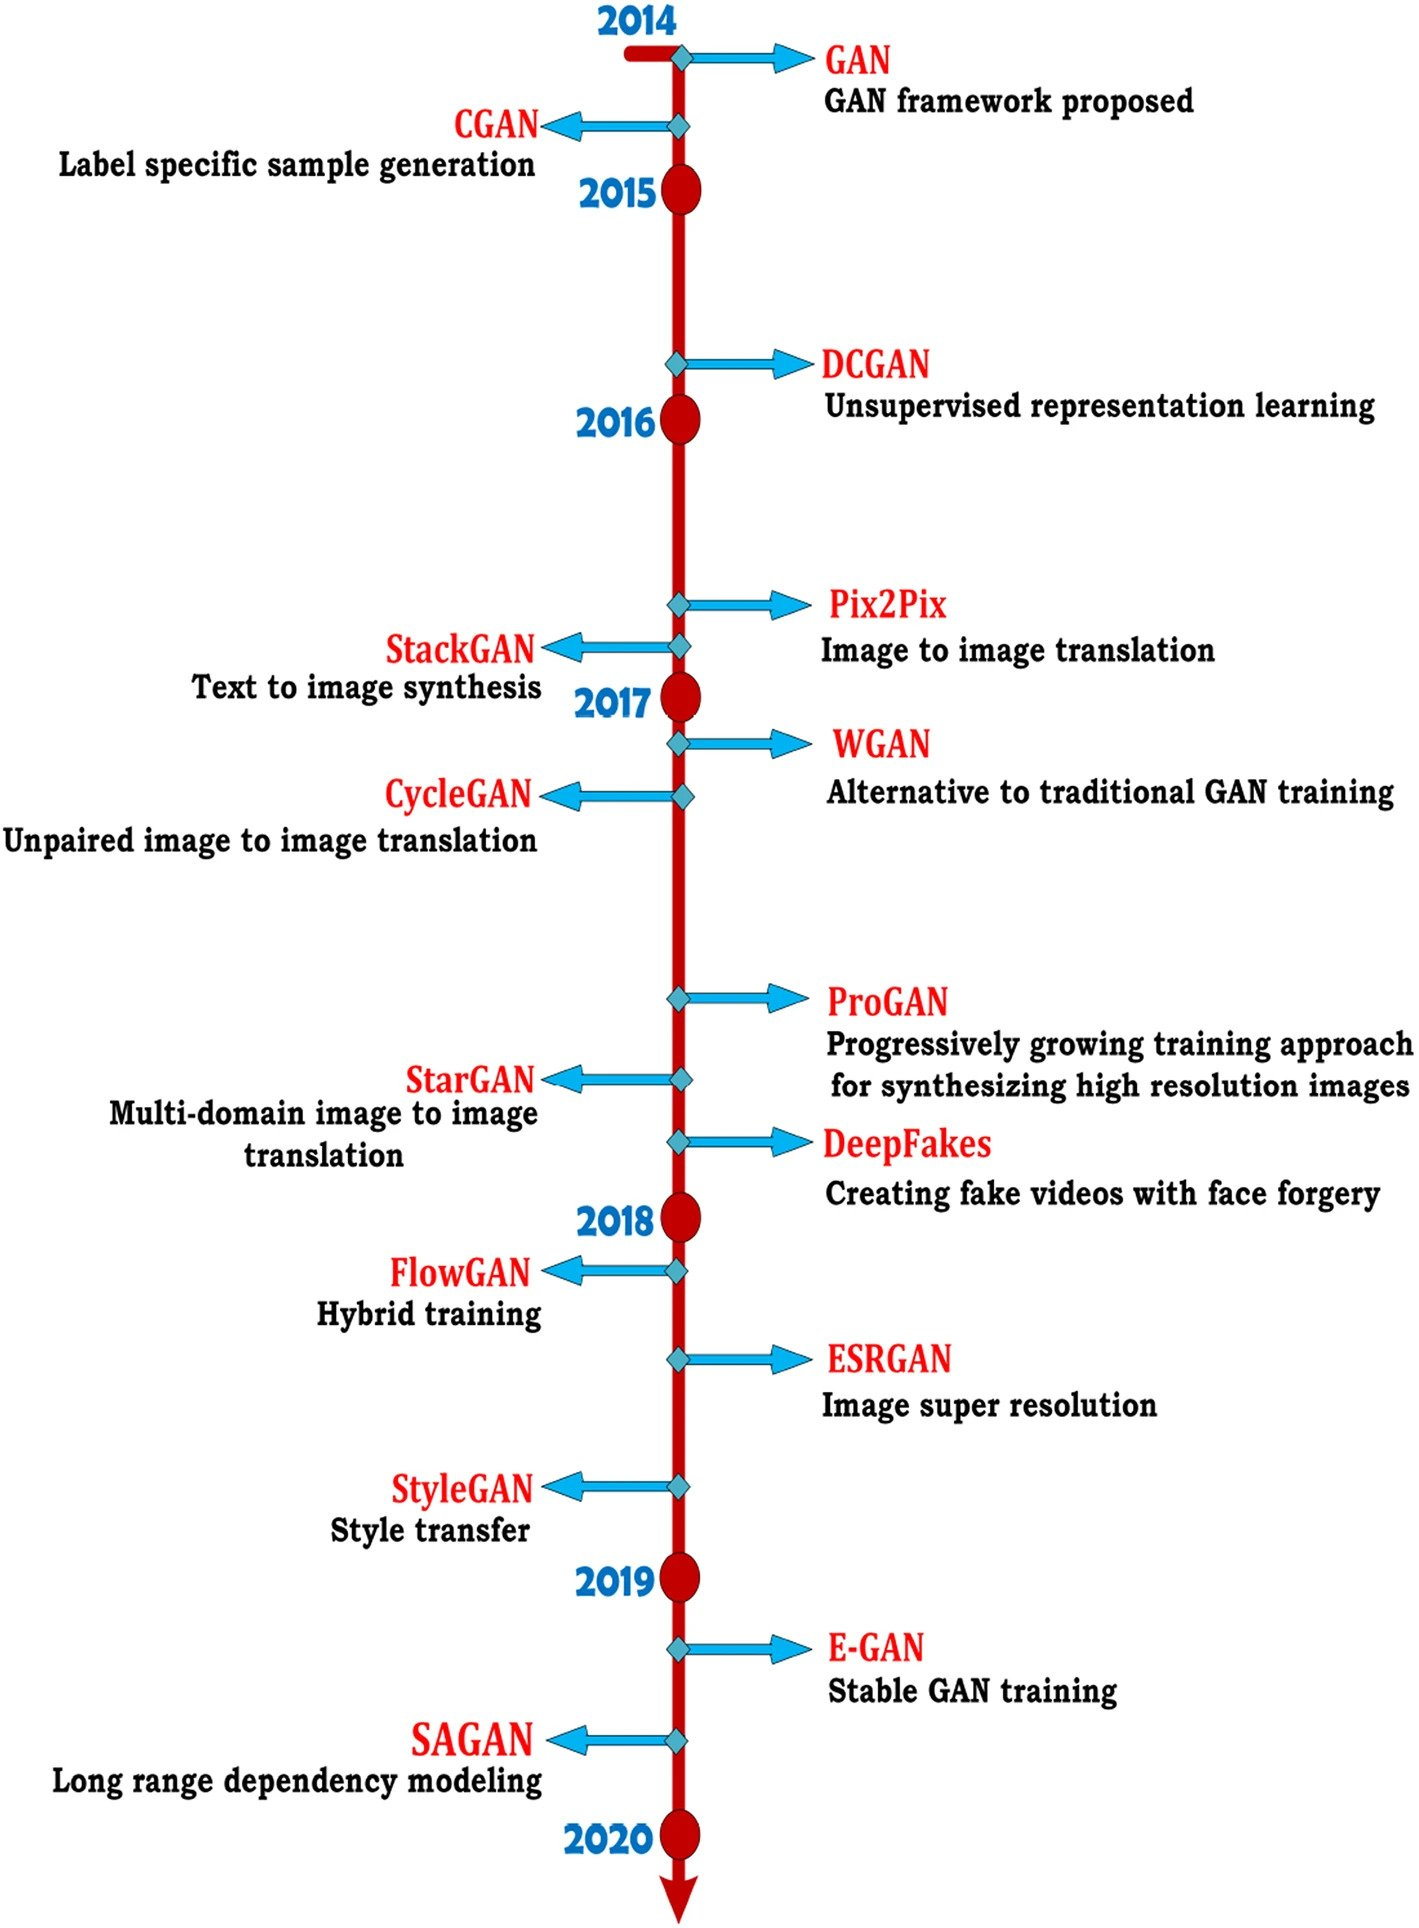
\includegraphics[scale=0.25]{images/relatedWorks/GANEvolution.jpg}
	    \caption[Evolution of \acp{GAN} Over the Years.]{Evolution of \acp{GAN} Over the Years\cite{PavanKumar.2021}.}
	    \label{fig:GANEvolution}
	    \end{center}
\end{figure}




Xudong Mao et al.\cite{mao2017squares} proposed another variant of \acp{GAN} called \acp{LSGAN}. ``The discriminator is hypothesized to be a classifier with the sigmoid cross-entropy loss function in regular \acp{GAN}. They realized, however, that the cross-entropy loss function can cause vanishing gradients during the learning process''\cite{mao2017squares}. Hence, the authors presented the \acp{LSGAN}, which uses the least-squares loss function for the discriminator to solve this problem. ``The fake samples are penalized by the least-squares loss function, which forces the generator to generate samples closer towards to the decision boundary''\cite{mao2017squares}. The authors evaluated \acp{LSGAN} using two datasets LSUN\cite{yu2016lsun} and HWDB1.0 (Handwritten Chinese Character Dataset)\cite{6065551}. When trained on the LSUN dataset\cite{yu2016lsun} they observed, the images generated by \acp{LSGAN} are of better quality than the ones generated by the two baseline methods, \acp{DCGAN}\cite{radford2016unsupervised} and EBGANs\cite{zhao2017energybased}. Also, when trained on the Handwritten Chinese Character Dataset, the generated characters were readable and clear. Another experiment was conducted to evaluate the stability of \acp{LSGAN} on a Gaussian mixture distribution dataset, which is designed in literature by Luke Metz et al.\cite{metz2017unrolled}. They train \acp{LSGAN} and regular \ac{GAN} on a 2D mixture of 8 Gaussian datasets using a simple architecture, where both the generator and the discriminator contain three fully-connected layers. ``It is observed that regular \acp{GAN} suffer from mode collapse. \acp{GAN} generate samples around a single valid mode of the data distribution. But \acp{LSGAN} learn the Gaussian mixture distribution successfully''\cite{mao2017squares}. Further, in this paper, for evaluating the stability, numerous comparison experiments are conducted and the results demonstrate that \acp{LSGAN} can generate higher quality images than regular \acp{GAN}, \acp{DCGAN}\cite{radford2016unsupervised}, and \acp{EBGAN}\cite{zhao2017energybased} and the learning process is stable compared to the regular \acp{GAN}.


Phillip Isola et al.\cite{isola2018imagetoimage} proposed \acp{cGAN} as a generic solution to numerous image-to-image translation problems. The authors wanted to provide a single solution for multiple types of image-to-image translation problems. For example, synthesizing photos from label maps\cite{cordts2016cityscapes}, reconstructing objects from edge maps\cite{zhu2018generative}\cite{6909426}, and colorizing images\cite{wesley2021colorizing}. ``\ac{cGAN} learns the mapping from the input image to output image along with a loss function to train this mapping. This allows using the same generic method to the distinct problems, that traditionally would require very different loss formulations''\cite{isola2018imagetoimage}. ``In \ac{cGAN} the generator uses U-Net-based architecture, the U-Net is an encoder-decoder with skip connections between mirrored layers in the encoder and decoder stacks\cite{ronneberger2015unet}. The discriminator uses a convolutional PatchGAN classifier, which only penalizes structure at the scale of image patches\cite{li2016precomputed}. Also, unlike unconditional \acp{GAN}, both the generator and discriminator observe the input images''\cite{isola2018imagetoimage}. Authors found ``L1 loss encourages less blurring compared to the L2 loss''\cite{isola2018imagetoimage}. Also combining L1 Loss and \ac{cGAN} (L1 + \ac{cGAN}) generates better results compared to combining Unconditional \ac{GAN} and L1 Loss (L1 + \ac{GAN}). ``The \ac{cGAN} appears to be more effective on the problem where the output is highly detailed or photographic''\cite{isola2018imagetoimage}. Authors have released \ac{cGAN} as the pix2pix software and mentioned, \ac{cGAN} has widespread applications, and it can be adopted without ease to solve different image-to-image translation problems without significant parameter modifications. The pix2pix software code is available at \href{https://github.com/phillipi/pix2pix.}{GitHub}. In figure \ref{fig:CGAN} the mapping from edges $\rightarrow$ photo transformation illustrated, and both generator and discriminator are conditioned on additional information like input edge map\cite{isola2018imagetoimage}.


\begin{figure}[H]
        \begin{center}
 	    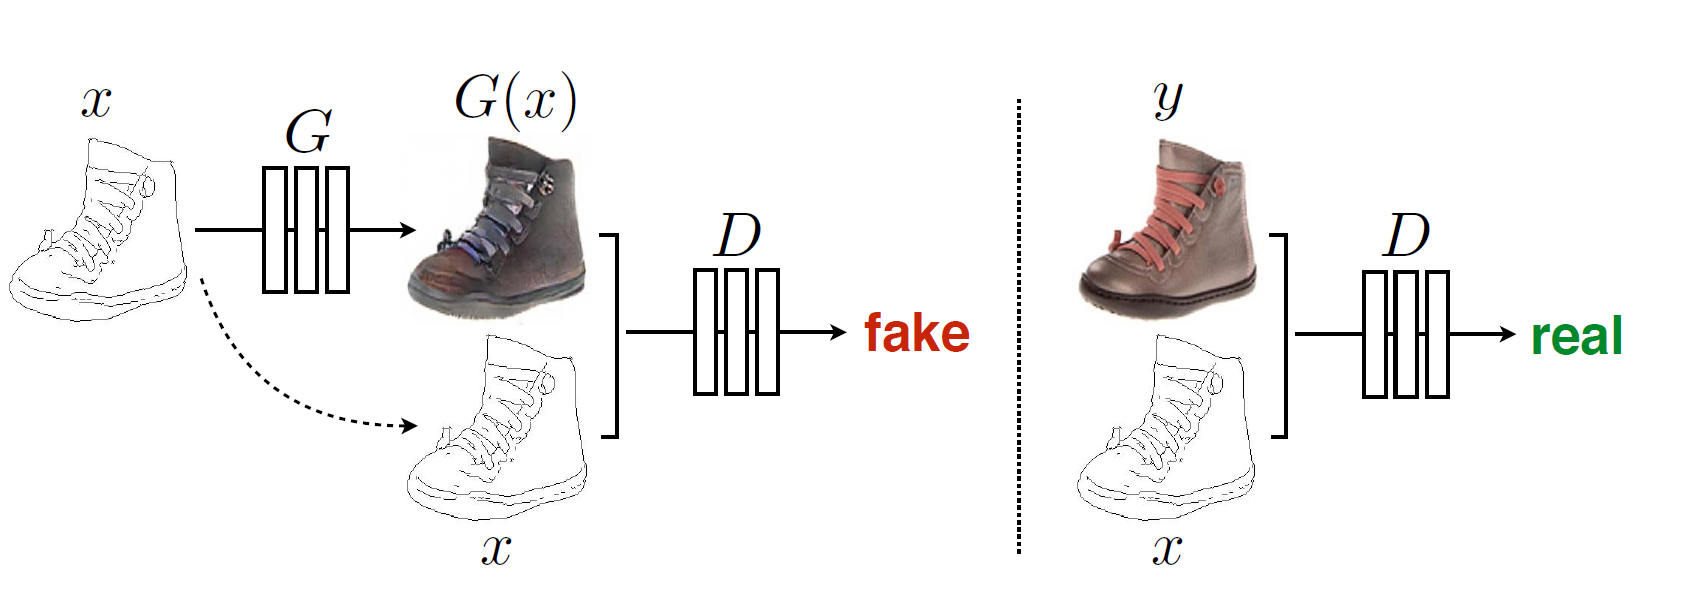
\includegraphics[scale=0.30]{images/relatedWorks/CGAN.png}
	    \caption[An illustration of training a \ac{cGAN} to map edges $\rightarrow$	 photo transformation.]{An illustration of the training a \ac{cGAN} to map edges $\rightarrow$ photo transformation. In \acp{cGAN}, both discriminator and generator observe the input edge map, unlike unconditional \acp{GAN}\cite{isola2018imagetoimage}.}
	    \label{fig:CGAN}
	    \end{center}
\end{figure}

Taesung Park et al.\cite{park2020contrastive} proposed \ac{CUT} for encouraging content preservation in unpaired image-to-image translation problems by maximizing the mutual information between input and output with patchwise contrastive learning\cite{oord2019representation}. Authors stated, ``In the patchwise contrastive learning for image-to-image translation, a generated output patch should appear closer to its corresponding input patch in comparison to other random patches present in the same input. To achieve patchwise contrastive learning, drawing patches internally from within the input image, rather than externally from other images in the dataset, forces the patches to better preserve the content of the input''\cite{park2020contrastive}. They demonstrated, ``the framework enables one-sided translation in the unpaired image-to-image translation setting while improving quality, consuming less memory, and reducing training time''\cite{park2020contrastive}. The prime advantage of this method is it does not require lots of memory\cite{8578491}\cite{he2020momentum} or specialized architecture\cite{henaff2020dataefficient}\cite{bachman2019learning}. The contrastive representation is formulated within the same image, hence this method can even be trained on single images, where each domain is having only a single image\cite{park2020contrastive}. The several prior methods like \ac{CycleGAN}\cite{zhu2020unpaired}, \ac{MUNIT}\cite{liu2018unsupervised}, \ac{DRIT}\cite{lee2019drit}, and \ac{GCGAN}\cite{fu2018geometryconsistent} were unable to achieve significant results compared to the \ac{CUT} method, on other hand, it often produced higher quality images and more accurate generations with light footprint in terms of training speed and GPU memory usage. Since \ac{CUT} method is one-sided, it is memory efficient and faster compared to prior baselines. Furthermore, the authors also introduced faster and lighter variant \ac{FastCUT}. \ac{FastCUT} also produces competitive results with even lighter computation cost of training. The code and models for \ac{CUT} are available at \href{https://github.com/taesungp/contrastive-unpaired-translation}{GitHub}.


\begin{figure}[H]
        \begin{center}
 	    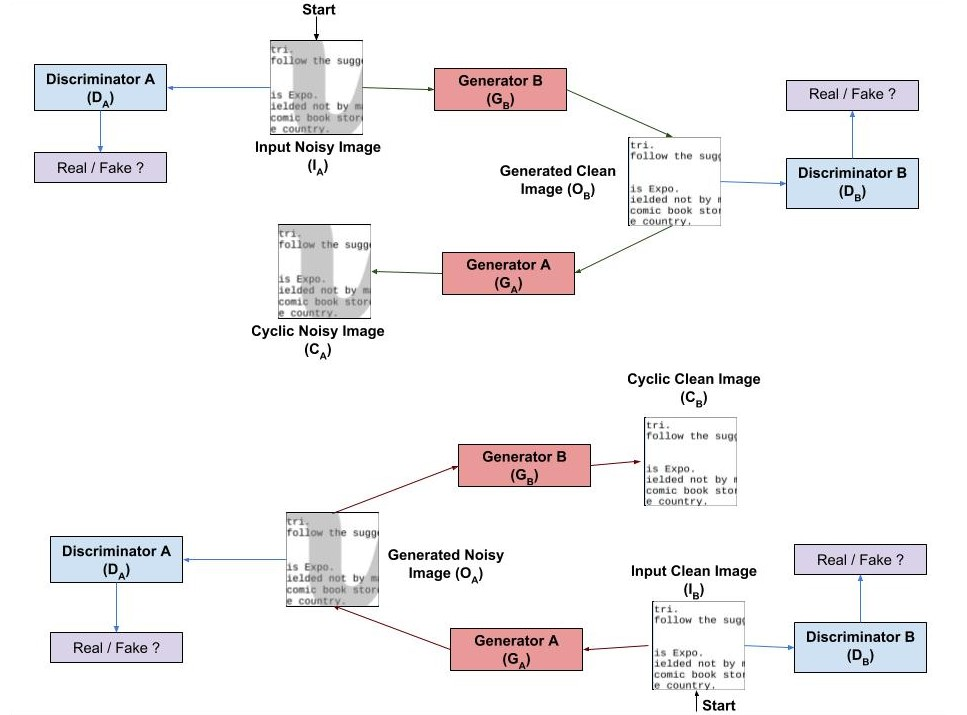
\includegraphics[scale=0.60]{images/relatedWorks/LearningToClean.jpg}
	    \caption[An illustration of \ac{CycleGAN} transforming the noisy document images into clean document images, and vice versa.]{An illustration of \ac{CycleGAN} transforming the noisy document images into clean document images, and vice versa. The generators $G_A$ and $G_B$ are responsible for the mapping of noisy images to clean images using cycle-consistency loss\cite{zhu2020unpaired}. The two discriminators $D_A$ and $D_B$ rejects samples generated by $G_A$ and $G_B$ respectively acting as an adversary\cite{sharma2019learning}.}
	    \label{fig:LearningToClean}
	    \end{center}
\end{figure}



Monika Sharma et al.\cite{sharma2019learning} are addressing ``a problem in the scanning process that often results in the introduction of blur due to camera motion, salt and pepper noise, or water markings, shake, wrinkles, coffee stains, or faded data. These artifacts pose many readability challenges to current text recognition algorithms and significantly degrade their performance''\cite{sharma2019learning}. ``The existing denoising techniques require a paired training dataset consisting of noisy documents paired with cleaned versions of the same document. However, in the real world, to generate clean documents from noisy versions, such a paired training dataset is not available to train a model''\cite{zhu2020unpaired}\cite{sharma2019learning}. Hence, the authors used \ac{CycleGAN} to transform noisy document images to clean document images and vice versa\cite{zhu2020unpaired}. ``\ac{CycleGAN} is a method to learn a mapping between two data distributions in the absence of paired training dataset''\cite{zhu2020unpaired}\cite{sharma2019learning}. They have compared the performance of \ac{CycleGAN} for document cleaning tasks with \ac{cGAN} by training them over the same dataset. The only difference was \ac{CycleGAN} trained using unpaired images and \ac{cGAN} trained using the paired images. They have used \ac{PSNR}\footnote{Peak Signal-to-Noise Ratio: \url{http://www.ni.com/white-paper/13306/en/} last access: \dcdate.} as a evaluation metric to evaluate the quality of transformed denoised images. Several experiments were performed on 4 separate public document datasets, one each for deblurring, watermark removal, background noise removal, and defading. Finally, they concluded ``\ac{CycleGAN} learns a more robust mapping from the space of noisy to clean documents compared to \ac{cGAN}''\cite{sharma2019learning}. The complete architecture of \ac{CycleGAN} for denoising documents illustrated in figure \ref{fig:LearningToClean}.


\begin{figure}[H]
        \begin{center}
 	    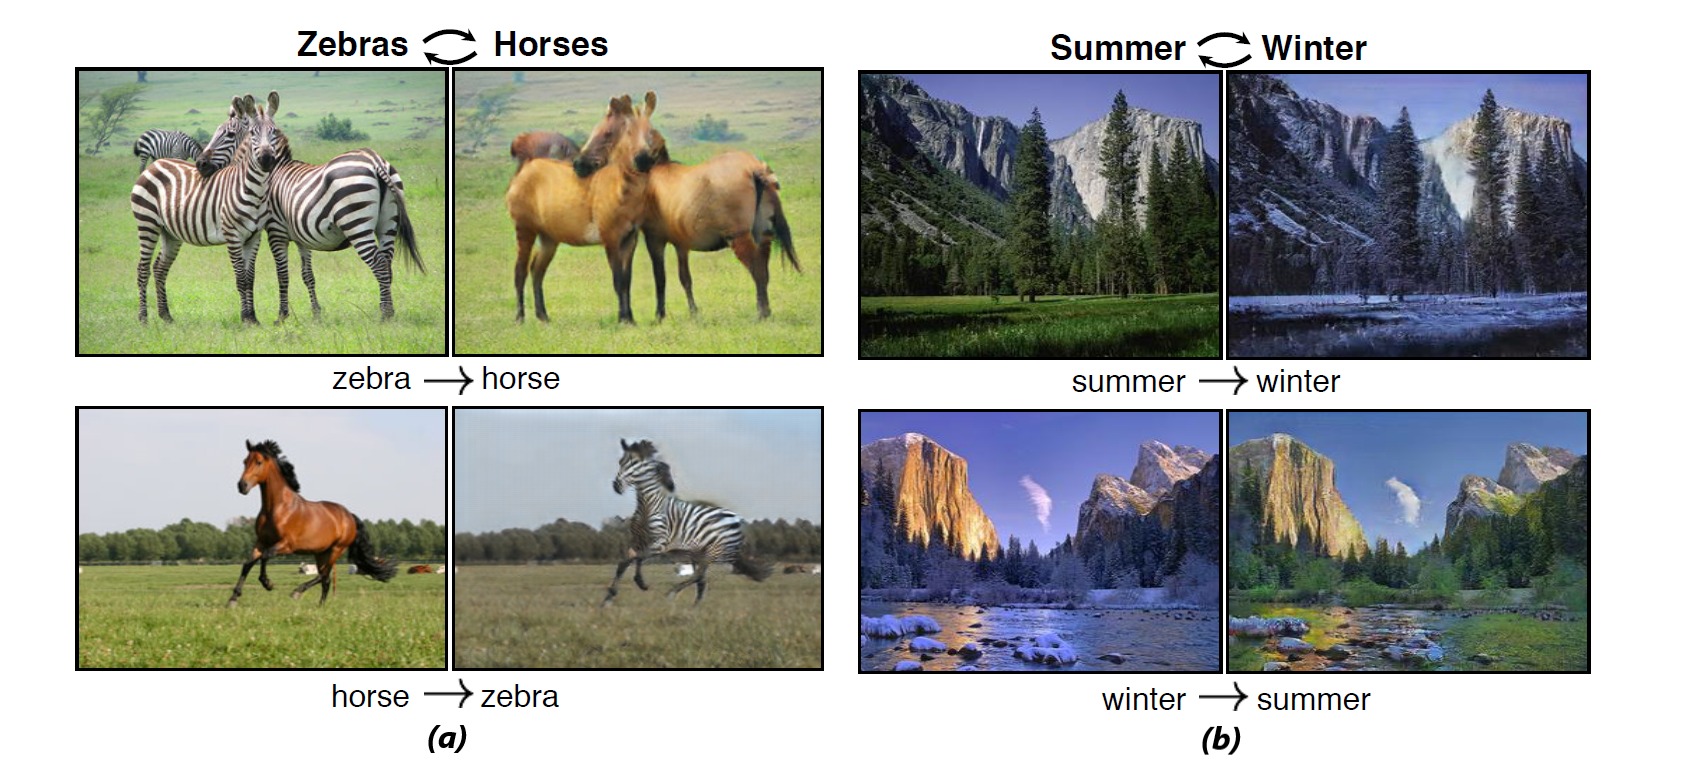
\includegraphics[scale=0.35]{images/relatedWorks/CycleGANExamples.png}
	    \caption[An illustration of \ac{CycleGAN} transforming an image from one into the other and vice versa.]{An illustration of \ac{CycleGAN} transforming an image from one into the other and vice versa. For example, zebra image transformed into horse image, and vice versa. The view of Yosemite mountains in summer transformed into winter, and vice versa\cite{zhu2020unpaired}.}
	    \label{fig:CycleganExamples}
	    \end{center}
\end{figure}



Jun-Yan Zhu et al.\cite{zhu2020unpaired} proposed \ac{CycleGAN} as an image-to-image translation method that can transform the images from source domain $X$ to target domain $Y$ in the absence of paired training dataset. ``This method learns to capture underlying characteristics of the collection of images in the source domain and figuring out how these characteristics could be transformed into the collection of images in the target domain, all in the absence of any paired training examples. In this method, the goal is to learn a mapping $G\ \colon X \rightarrow Y$ so that the generated distribution of images $G(X)$ matches the target distribution $Y$ using an adversarial loss. However, the adversarial losses alone are not sufficient to map the images from the source domain to the target domain. Hence, authors introduced inverse mapping $F\ \colon Y \rightarrow X$ to introduce a cycle-consistency loss to enforce $F(G(X))\approx X$, and vice versa to regularize the output and keep it highly under-constrained''\cite{zhu2020unpaired}. 


Authors also introduced identity mapping loss which helps to preserve the color of input images. 




The several prior methods like Bi-GAN/ALI [\cite{donahue2017adversarial},\cite{dumoulin2017adversarially}], CoGAN\cite{liu2016coupled}, SimGAN\cite{shrivastava2017learning} were unable to achieve compelling results. The \ac{CycleGAN} method, on other hand, can produce images that are often of similar quality to the fully supervised pix2pix\cite{isola2018imagetoimage}. Authors provide both \href{https://github.com/junyanz/pytorch-CycleGAN-and-pix2pix}{PyTorch} and \href{https://github.com/junyanz/CycleGAN}{Torch} implementations. In figure \ref{fig:CycleganExamples} examples of \ac{CycleGAN} transforming an image from one into the other and vice versa illustrated.


Chris Tensmeyer et al.\cite{8978087} realized solving binarization tasks using deep learning models is very challenging. It is due to the scarcity of large quantities of labeled data available to train such models. There have been efforts to create synthetic data for binarization using image processing techniques but, they generally lack realism\cite{8978087}. Hence, authors proposed DGT-CycleGAN to produce realistic synthetic data using an adversarially trained image-to-image translation model\cite{8978087}. Authors modified the \ac{CycleGAN} model to be conditioned on the ground truth binarization mask as it transforms images from the source domain of synthetic images to the target domain of real images\cite{8978087}. They found modifying the discriminator to condition on the binarization \ac{GT} leads to increased realism and better agreement between the \ac{GT} and the produced image\cite{8978087}.  Authors pretrained deep learning models on realistic synthetic datasets generated by \ac{CycleGAN}, DGT-CycleGAN, and image compositing\cite{8978087}. They found pretraining a model on realistic synthetic data generated by the DGT-CycleGAN model achieves the best performance for solving binarization tasks compared to data generated by \ac{CycleGAN} and image compositing\cite{8978087}.


Also, they evaluated both pretrained only and finetuned models on each of the \ac{DIBCO} datasets\footnotemark. 

Finetuning a model on \ac{DIBCO} dataset after pretraining on the realistic synthetic images generated by the DGT-CycleGAN has lead to a 13\% reduction of F-measure error compared to no pretraining. Authors concluded, pretraining deep neural networks on the realistic synthetic data generated using DGT-CycleGAN lead to better predictive performance both before and after finetuning on real data.


\footnotetext{\ac{DIBCO} 2019: \url{https://vc.ee.duth.gr/dibco2019/} last access: \dcdate}


\section{Discussion}\label{rwdiscussion}
Over the years, \acp{GAN} have evolved to solve different kinds of problems. The evolution of the \acp{GAN} is illustrated in the figure \ref{fig:GANEvolution} using a timeline diagram. \acp{GAN} suffer from unstable training, vanishing gradients problem, and mode collapse. Consequently, Martin Arjovsky et al.\cite{arjovsky2017wasserstein} proposed \ac{WGAN} to solve problems with \acp{GAN}. \acp{WGAN} improve the stability of learning, get rid of problems like mode collapse, and provide meaningful learning curves useful for debugging and hyperparameter searches. Although the implementation of \ac{WGAN} is straightforward, the theory behind it is heavy and requires some hack, for example, Weight Clipping \cite{gulrajani2017improved}. Hence, Xudong Mao et al.\cite{mao2017squares} proposed a simple and more intuitive method compared to \ac{WGAN}, called \ac{LSGAN}. First, \acp{LSGAN} are able to generate higher quality images than regular \acp{GAN}. Second, \acp{LSGAN} perform more stable during the learning process. Moreover, Jun-Yan Zhu et al.\cite{zhu2020unpaired} proposed \ac{CycleGAN}. It is an unsupervised image-to-image translation approach. Compared to \acp{GAN}, \acp{CycleGAN} can deal more meticulously with the problems like unstable training, vanishing gradients problems, and mode collapse. Also, they described that \ac{CycleGAN} has outperformed existing baselines as Bi-GAN/ALI [\cite{donahue2017adversarial},\cite{dumoulin2017adversarially}], CoGAN\cite{liu2016coupled}, and SimGAN\cite{shrivastava2017learning}. Furthermore, Monika Sharma et al.\cite{sharma2019learning} proclaimed  \ac{CycleGAN} can transform noisy document images into denoised and clean document images to achieve image-to-image translation. They have also compared the performance of the developed image-to-image application with \ac{cGAN} and demonstrated \ac{CycleGAN} had outperformed \ac{cGAN}. Chris Tensmeyer et al.\cite{8978087} proposed DGT-CycleGAN, a modified version of \ac{CycleGAN}, which is adequate to translate images from the domain of synthetic images to the domain of real images to solve binarization tasks. Moreover, Taesung Park et al.\cite{park2020contrastive} proposed \ac{CUT}. They have demonstrated that \ac{CUT} is a better, faster, and memory-efficient approach to perform unsupervised image-to-image translation. It has outperformed \ac{CycleGAN}\cite{zhu2020unpaired}, \ac{MUNIT}\cite{liu2018unsupervised}, \ac{DRIT}\cite{lee2019drit}, and \ac{GCGAN}\cite{fu2018geometryconsistent}. However, due to time constraints, multiple available references, and code repositories, \ac{CycleGAN} has been a choice for this thesis and research to perform unsupervised image-to-image translation.


\section{Conclusion}\label{rwconclusion}

The image-to-image translation is a classic example of computer vision and computer graphics problems. In which the goal is to learn the mapping between a source image and target image using a training set of aligned image pairs. Although, for many tasks, aligned or paired training data will not be available. Also, collecting and annotating paired document images is tedious, difficult, time-consuming, and costly. This thesis is attempting to close a domain gap between synthetic document images and real document images in the absence of paired training data. The thesis proposes an image-to-image translation application to transform synthetic document images into realistic document images to perform domain adaptation, by closing the gap between synthetic data distribution and real data distribution. Ultimately, a large amount of realistic annotated set of document images can be generated using this application. Furthermore, they can be used to improve real document image classification. Also, in case, if a classifier is trained using such generated realistic document images, it can fasten the process of labeling the new annotated or unlabeled real document images. As per the above literature survey [\cite{zhu2020unpaired},\cite{sharma2019learning}] and problem statement, in this thesis \ac{CycleGAN} is a decided method to transform synthetic document images into realistic document images in the absence of paired training data. Hence, the proposed image-to-image translation application is realized using \ac{CycleGAN}.





%Authors considered evaluation metrics like \ac{AMT} perceptual studies, FCN-score\cite{isola2018imagetoimage}, and semantic segmentation metrics to compare the quality of generated images against other baseline. 
%The evaluation metrics like \ac{FID}\cite{heusel2018gans} and semantic segmentation scores are used to compare the quality of generated images using \ac{CUT} method. 

%Authors performed multiple experiments during ablation studies using evaluation metrics like, \ac{AMT} perceptual study, FCN-Score, and semantic segmentation metrics. 

%In this thesis, \ac{CycleGAN} is used to perform domain adaptation. Discussion about the loss functions has been carried out in-depth in Chapter \ref{methodology}.
%is combined with \ac{LSGAN}, in which the discriminator model is updated using a least-squares loss (L2 Loss).
%The thesis aims to develop an image-to-image translation application to transform synthetic document images into realistic document images. The thesis aims to develop an image-to-image translation application to transform synthetic document images into realistic document images to perform domain adaptation. Ultimately, a large amount of realistic annotated set of document images can be generated using this application.




